\section{实验步骤}
\subsection{利用fork系统调用创建出指定进程树}
我在programs文件夹中创建如代码\ref{lst:procTest}所示源文件。并依次在命令行中使用make all和make qemu命令。程序输出如图\ref{ws2}所示。
\begin{listing}[htbp]
    \begin{minted}{c}
#include<stdio.h>
#include<sys.h>
int main1()
{
    //2#
    int ws = 2;
    int i,j,k,pid,ppid;
    if(fork())
    {
        //2#
        sleep(2);
        for(k=1;k<6;k++)
        {
            printf("%d %d; ",k,getppid(k));
        }
        printf("\n");
    }
    else
    {
        //3#
        if(fork())
        {
            //3#
            if(fork())
            {
                //3#
                pid = getpid();
                ppid = getppid(pid);
                for(k=0;k<ws;k++)
                {
                    i = wait(&j);
                    printf("Process %d#:My child %d is finished with exit status %d\n",pid,i,j);
                }
                printf("Process %d# finished: My father is %d\n",pid,ppid);
                exit(ppid);
            }
            else
            {
                //5#
                pid = getpid();
                ppid = getppid(pid);
                printf("Process %d# finished: My father is %d\n",pid,ppid);
                exit(ppid);
            }
        }
        else
        {
            //4#
            pid = getpid();
            ppid = getppid(pid);
            printf("Process %d# finished: My father is %d\n",pid,ppid);
            exit(ppid);
        }
    }
}
    \end{minted}
    \caption{procTest.c}\label{lst:procTest}
\end{listing}
\subsection{修改程序使得父进程先于所有子进程结束}
将代码\ref{lst:procTest}中的变量初值改为0后,得到的程序输出如图\ref{ws0}所示。
\subsection{修改程序使得父进程先于部分子进程结束}
将代码\ref{lst:procTest}中的变量初值改为1后,得到的程序输出如图\ref{ws1}所示。

为了进一步分析调度过程,我通过单步调试的方式确定了操作系统运行\texttt{procTest}的入口位于\texttt{shell/ExecuteCommand.c}中的 \texttt{ExecuteTCOM}函数体内 ,主要代码如代码\ref{lst:ExecuteCommand}所示。

\begin{listing}[htbp]
    \begin{minted}{c}
int child = fork();
int dead = -1;
if ( child != 0 ) /* parent */
{
    if ( (node->params & FAND) == 0 ) /* need wait */
    {
        while( wait(&state)!= child);
        //wait(&state);
    }
}
    \end{minted}
    \caption{ExecuteCommand.c}\label{lst:ExecuteCommand}
\end{listing}

从中可以看出,命令行程序实际上就是1\#进程,当我们在其中输入所要运行的程序时,它便通过调用 \texttt{fork()}来创建出相应的进程。由于过程中没有
入睡,所以会先返回父进程,也就是命令行程序,然后在正常情况下进入条件分支,如果需要等待,则循环执行 \texttt{wait()},退出循环的条件是返回代码为
命令行创建的子进程的进程号。

作如图\ref{fig:ExecuteCommand}所示的更改,编译后运行,可以得到如图\ref{fig:after}的输出,佐证了上述说明。可以看到,程序运行后前3\#,5\#进程不存在。
程序运行结束后,除了0\#进程存在外,还有1\#,3\#,5\#进程存在,但是其中3\#,5\#进程在程序运行前不存在,所以只有1\#进程有可能是命令行程序对应的进程。

\begin{figure}[!htbp]
    \centering
    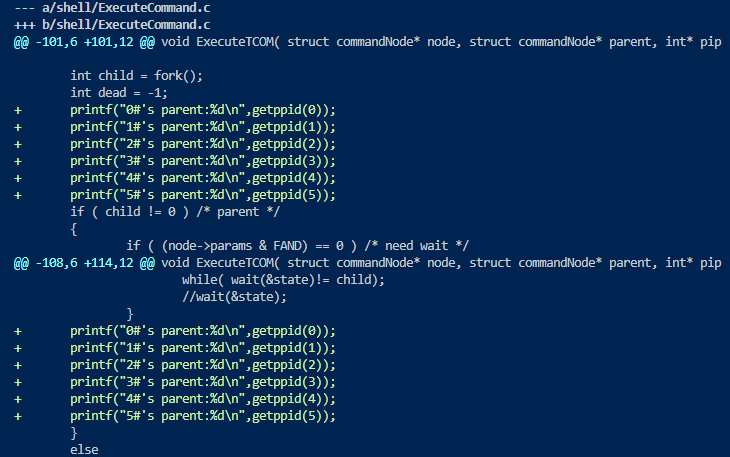
\includegraphics[width=\textwidth]{images/ExecuteCommand.png}
    \caption{对\texttt{ExecuteCommand.c}的更改}\label{fig:ExecuteCommand}
\end{figure}

\begin{figure}[!htbp]
    \centering
    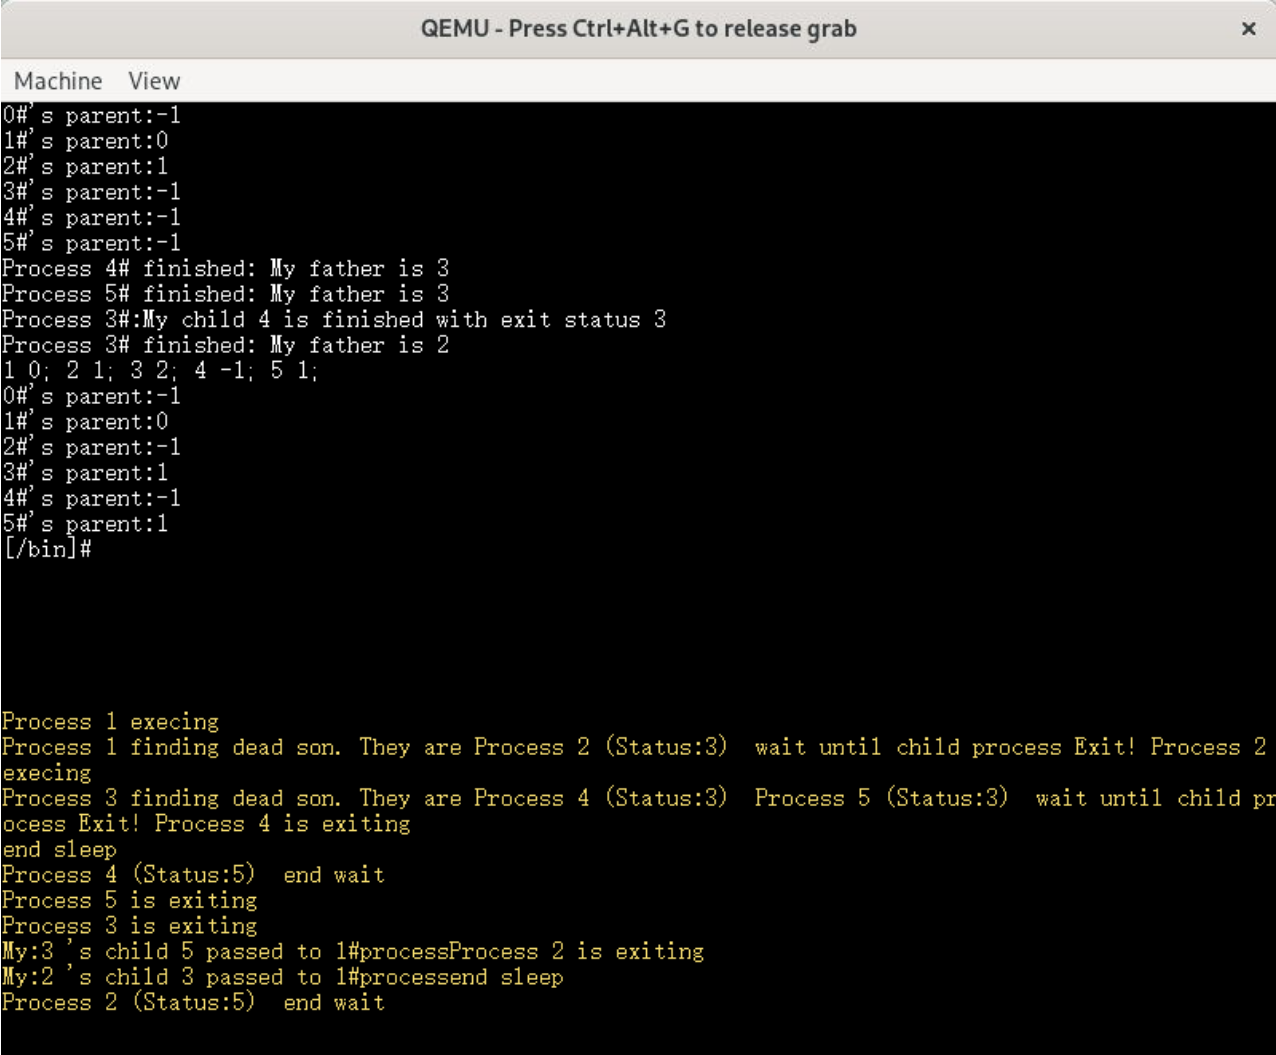
\includegraphics[width=\textwidth]{images/after.png}
    \caption{更改后的输出}\label{fig:after}
\end{figure}

\texttt{ws=1}时程序\texttt{procTest}运行过程中的关键内核态函数调用情况以及调度情况如表\ref{table:ws1}所示。

4\#和5\#进程在终止时能找到自己的父进程为3\#进程的原因是此时3\#进程还未终止。4\#进程终止时,唤醒了因为 \texttt{wait()}入睡的父进程3,并被回收,从而最终的打印结果中显示父进程为-1;
5\#进程终止时,由于父进程3不处于由 \texttt{wait()}引起的睡眠状态,所以未能被回收;3\#进程终止时,将仍存在的子进程5的父进程更改为进程1,同时由于自己的父进程2不处于由 \texttt{wait()}引起的睡眠状态,所以未能被回收;
进程3在完成\texttt{procTest}前的父进程仍为进程2,而当完成运行时自动调用\texttt{exit()},唤醒了由于\texttt{wait()}入睡的父进程1,并将2\#进程回收,同时将未被回收的子进程3的父进程设置为1。
由于回收进程2时返回的状态码符合循环终止条件,进程1不再调用\texttt{wait()}。因此进程5在 \texttt{procTest}运行结束前后的父进程均为1,
只有当后续进程1调用\texttt{wait()}函数时,才有可能在线性扫描时扫描到该子进程,并将其回收(3\#进程也未被回收,会先扫描到3\#进程)。

从图\ref{fig:after}中也可以看出,执行完\texttt{procTest}后,3\#,5\#进程的父进程仍为进程1。


\subsection{修改程序使得子进程能够抢占父进程}

之所以在4.1-4.3的实验中,父进程3\#进程始终没有被抢占,是因为3\#进程没有执行过计算任务,运行时间短,没有入睡也没有唤醒高优先级的进程,使得\texttt{fork}末尾处并没有设置\texttt{RunRun},从而没有
调用\texttt{Swtch}函数,提供被抢占的机会。


如果3\#进程不执行\texttt{wait},可以被子进程抢占的时机就是两处\texttt{fork}返回处后的例行调度。为了在例行调度中进行抢占,先前态为用户态的条件已经满足,还需要满足
$RunRun!=0$的条件。为此,可以通过三种方法达成:1)让3\#进程运行足够长时间,使得在\texttt{fork}末尾的\texttt{setPri}中p\_pri上升,从而设置RunRun;2)
让3\#进程入睡,从而由于睡眠时的优先数<100,重算时必定会设置RunRun;3)让\#3相应中断,唤醒更高优先级的进程,从而在\texttt{SetRun}中设置RunRun。其中,第一种方式可以通过调整代码的方式来实现。

为了复现实验指导书中的图6的结果,作如图\ref{fig6change}中的修改。主要修改之处是在进程3开始处增加计算任务,以提高其$p\_cpu$,从而在创建4\#进程后的\texttt{SetPri}中更新\texttt{RunRun}。
将\texttt{sleep(2)}改为\texttt{sleep(5)}的原因是为了避免2\#进程在3\#进程完成计算任务之前被唤醒。运行结果如图\ref{fig6}所示。

\begin{figure}[!htbp]
    \centering
    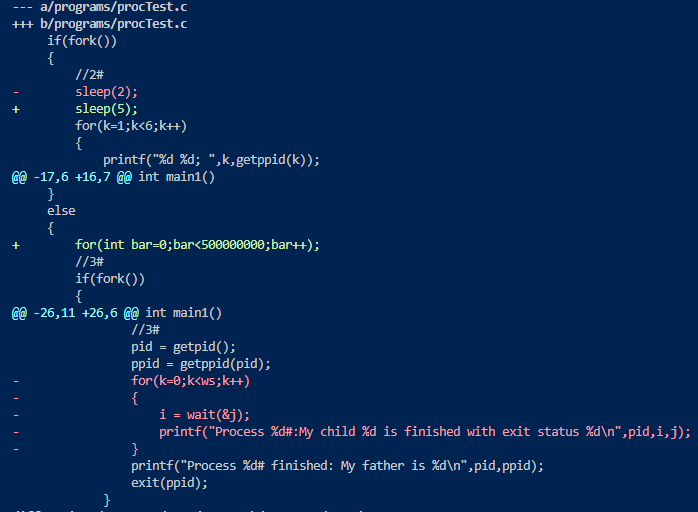
\includegraphics[width=\textwidth]{images/fig6change.png}
    \caption{父进程创建5\#之前被抢占}\label{fig6change}
\end{figure}

创建4\#进程和5\#进程时各进程的状态分别如图\ref{fork4},\ref{fork5}所示。

程序\texttt{procTest}运行过程中的关键内核态函数调用情况以及调度情况如表\ref{table:fig6}所示。

\begin{figure}[!htbp]
    \centering
    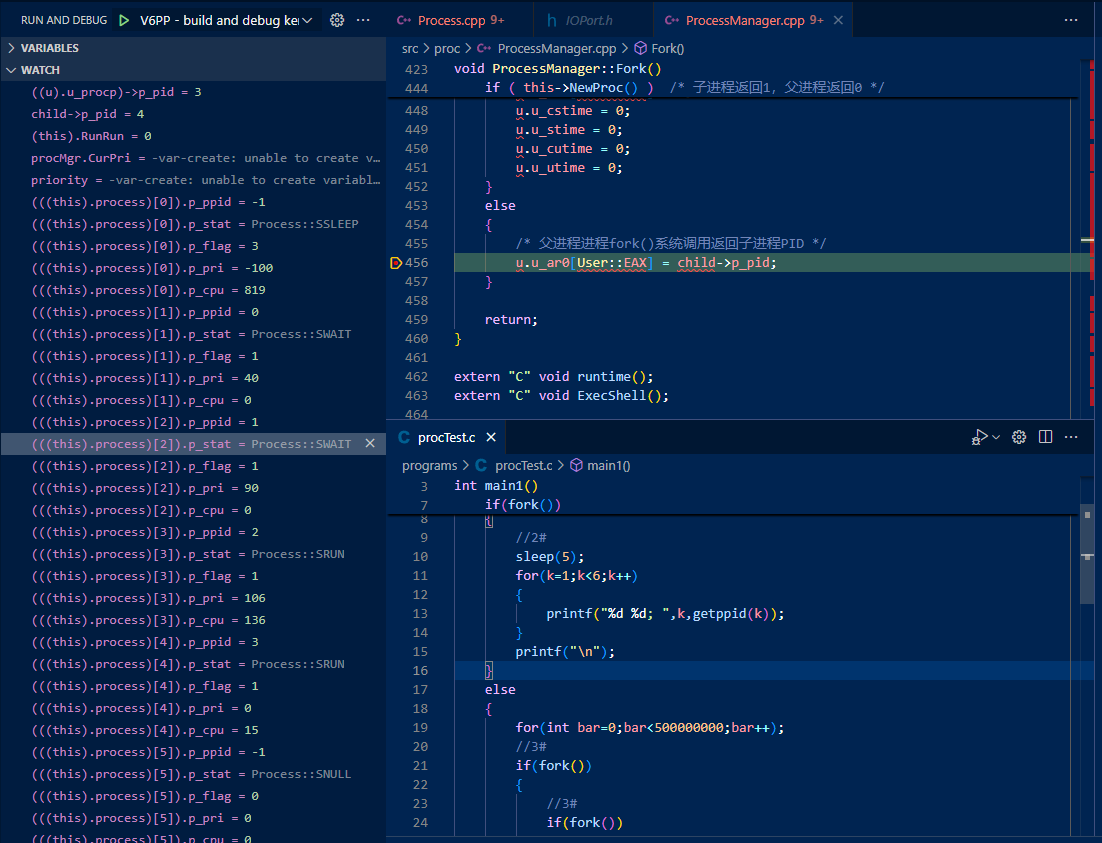
\includegraphics[width=\textwidth]{images/fork4.png}
    \caption{创建4\#进程时各进程的状态}\label{fork4}
\end{figure}

\begin{figure}[!htbp]
    \centering
    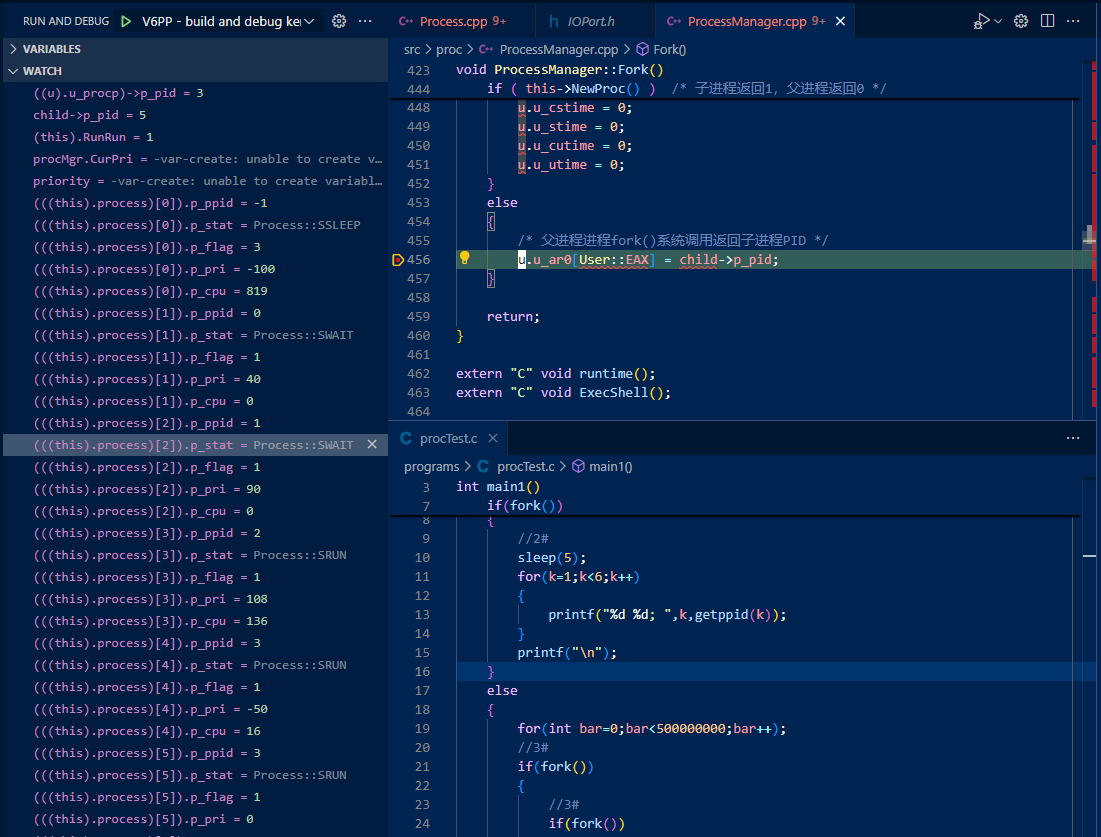
\includegraphics[width=\textwidth]{images/fork5.png}
    \caption{创建5\#进程时各进程的状态}\label{fork5}
\end{figure}

实验指导书中图6的输出解释如下:由于3\#进程执行运算任务导致$p\_cpu$增加,所以在创建4\#进程后\texttt{fork},会调用\texttt{Swtch},并被4\#进程抢占。
从而4\#进程先终止,由于其父进程3并未调用\texttt{wait},所以4\#进程并未被回收。然后3\#进程上台,创建进程\#5,由于上台期间并未执行计算任务,并不会设置\texttt{RunRun},
从而不会被5\#进程抢占。因此,之后进程3\#终止,并将其子进程4,5的父进程设为1\#进程。同时由于3\#进程的父进程2并未调用\texttt{wait},所以进程3\#也未被回收。然后5\#进程上台并终止,
由于其父进程1处于因为调用\texttt{wait}而进入的睡眠状态,所以1\#进程被唤醒,并回收5\#进程。由于得到的状态码不符合循环终止条件,1\#进程再次
调用\texttt{wait},并于其中回收进程4\#进程。
状态码仍不满足循环终止条件,1\#进程再次调用\texttt{wait}并入睡。最终2\#进程上台,打印结果然后终止,将3\#进程的父进程设置为1\#进程。
1\#进程上台,线性扫描至2\#进程并将其回收,由于满足循环终止条件,所以不再调用\texttt{wait}。

为了复现实验指导书中的图7的结果,在图\ref{fig6change}的基础上作如图\ref{fig7change}中的修改。唯一修改之处在于让父进程创建4\#进程之后、创建5\#之前执行计算任务。
程序运行结果如图\ref{fig7}所示。

\begin{figure}[!htbp]
    \centering
    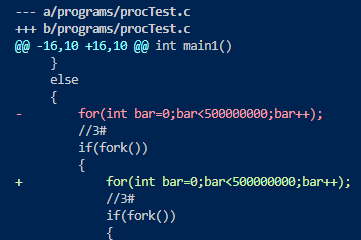
\includegraphics[scale=1]{images/fig7change.png}
    \caption{父进程创建5\#之后被抢占}\label{fig7change}
\end{figure}

创建4\#进程和5\#进程时各进程的状态分别如图\ref{2fork4},\ref{2fork5}所示。

程序\texttt{procTest}运行过程中的关键内核态函数调用情况以及调度情况如表\ref{table:fig7}所示。

\begin{figure}[!htbp]
    \centering
    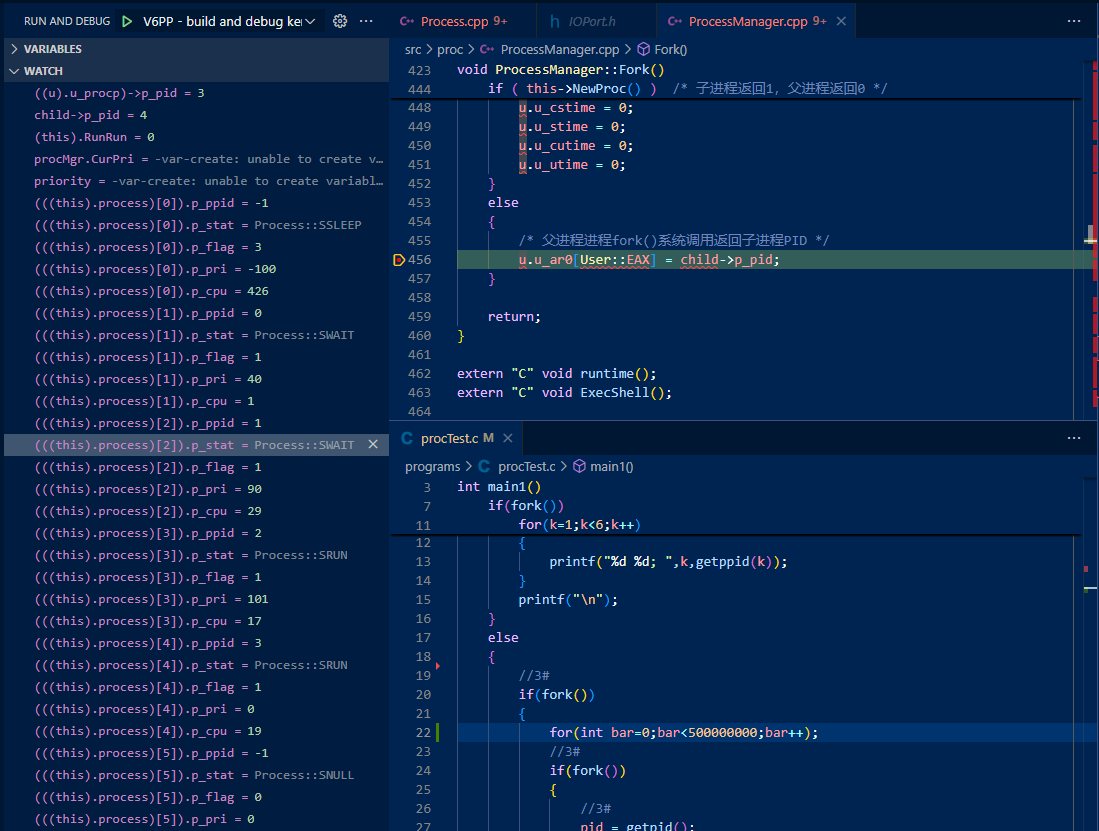
\includegraphics[width=\textwidth]{images/2fork4.png}
    \caption{创建4\#进程时各进程的状态}\label{2fork4}
\end{figure}

\begin{figure}[!htbp]
    \centering
    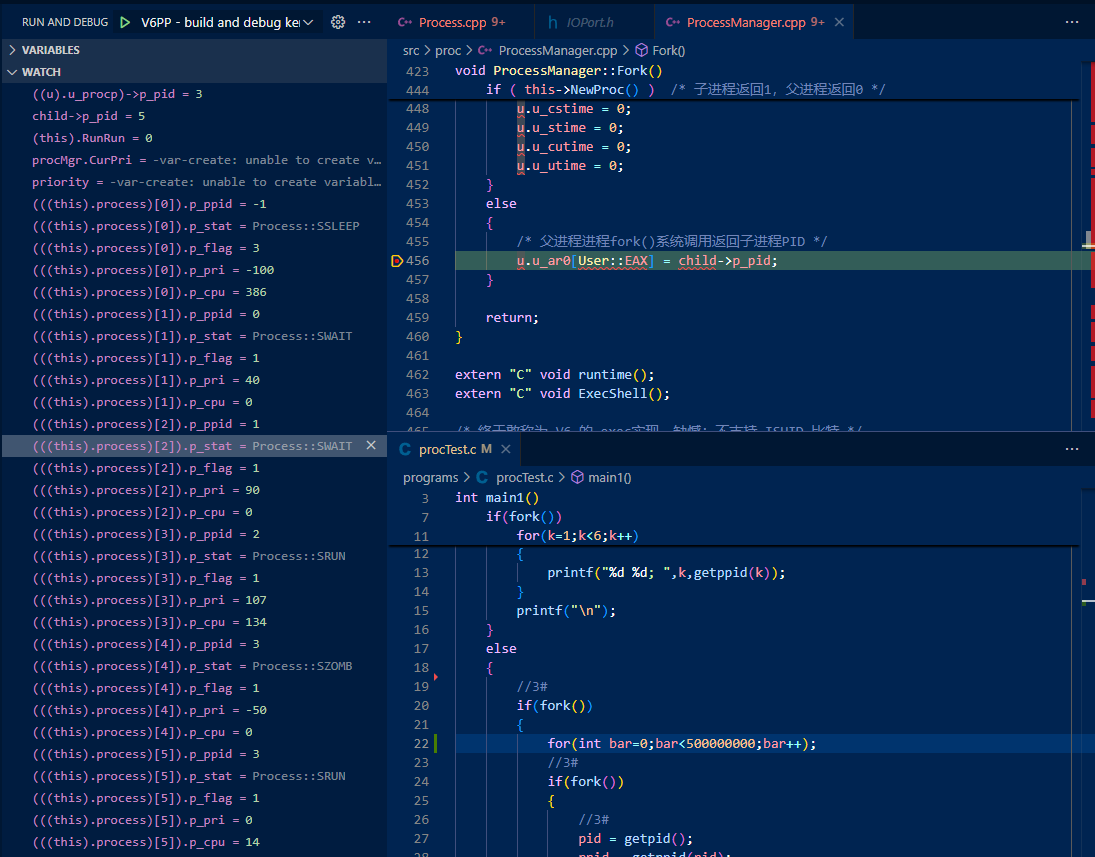
\includegraphics[width=\textwidth]{images/2fork5.png}
    \caption{创建5\#进程时各进程的状态}\label{2fork5}
\end{figure}

实验指导书中图7的输出解释如下:
3\#进程创建完4\#进程后未被抢占,并执行计算任务,然后创建5\#进程,之后才被抢占。最终4\#进程先上台返回用户态并退出。由于4\#进程的父进程3并未调用\texttt{wait},所以进程4\#未被回收。
然后由于5\#进程未执行过计算任务,重算优先级后也比3\#进程优先,所以上台运行并退出。类似的,由于5\#进程的父进程3并未调用\texttt{wait},所以进程5\#未被回收。
接着3\#进程上台并退出,将子进程4,5的父进程都设为1\#进程。同样,由于3\#进程的父进程2并未调用\texttt{wait},所以进程3\#未被回收。
最后,2\#进程上台,打印结果,并退出,同时将子进程3的父进程更新为1。由于2\#父进程1处于因为调用\texttt{wait}而进入的睡眠状态,所以1\#进程上台,线性扫描至2\#进程并将其回收,由于满足循环终止条件,所以不再调用\texttt{wait}。
